%\clearpage
\chapter{Kravspesifikasjon}
Vi skal få inn en tjeneste under et allerede eksisterende rammeverk. Med det må vi beskrive de kravene som må opprettholdes for at vi skal kunne få en suksessfull integrering med ny autentisering. Vi skal også beskrive detaljert hendelsesløpet for en autentisering innenfor rammeverket, eksisterende og det vi vil integrere. \newline \newline
Allerede eksisterende materiale vi kan se på er dokumentasjon på Openstack keystone-modulen og Feide-dokumentasjon.

\section{Brukerbeskrivelse}
\subsection{Omgivelser}
Som nevnt tidligere, så skal autentiseringstjenesten integreres. Det skal skje på et allerede eksisterende system, som allerede har en annen autentiseringstjeneste. Selve Openstack-systemet samkjøres mellom flere servere. Det er stykket opp i moduler for ytelse og funksjonalitet. Den modulen vi skal jobbe på er “Controller noden”, den kjører noen moduler som vi skal jobbe med og derfor må sette oss ekstra nøye inn i.

\begin{description}
	\item{\tab •} Horizon - Webinterfacet til Openstack-systemet. Der er brukergrensesnittet som brukes for å kunne lage, endre, slette og kjøre VM-ene, det er også her innloggingen ligger.
	\item{\tab •} Keystone - Tar seg av hvilke prosesser og VM-er som tilhører hvem. Derfor har også den en finger med i autentiseringen.
\end{description}

\subsection{Systemets brukere}
Det er tre grupper med brukere mot tjenesten vi skal integrere. De har alle forskjellige roller og autoritet innen systemet.

\begin{description}
	\item{\tab •} Studenter/brukere - De har kun lov til å kunne lage, endre, slette og bruke VM-er. De har også restriksjoner på ytelse og mengde plass som kan brukes.
	\item{\tab •} Ansatte - Forskjellen fra studentene er at de ansatte har ikke restriksjon på ytelse og mengde data.
	\item{\tab •} It-tjenesten - Gruppen som har mest tilgang, men av den praktiske grunn at de har vedlikeholdsarbeidet. De har også rettigheter som de overnevnte.
\end{description}

Opplæringen ved å bruke tjenesten er minimal. Vi skal jobbe med innloggingen. Noe absolutt alle har vært borti før, med tanke på at det er noe av det første du må gjøre når du kommer til HiG.

\newpage
\subsection{User stories}
\subsection{Primærmål}
\begin{table}[H]
	\begin{tabular}[Figur 2]{| p{2cm} p{9cm} |}
		\hline \textbf{Stikkord} & logge inn på domene \\
		\hline \textbf{Beskrivelse} & Brukeren vil at man skal kunne skrive inn et gitt domene og komme til log in-skjermen. I dette tilfelle er domene allerede ordnet: skyhigh.hig.no.
	\end{tabular}
\end{table}

\begin{table}[H]
	\begin{tabular}[Figur 2]{| p{2cm} p{9cm} |}
		\hline \textbf{Stikkord} & logge in med Feide\\
		\hline \textbf{Beskrivelse} & Kunden vil at brukeren må logge seg inn ved å bruke eksisterende brukernavn og passord. 
	\end{tabular}
\end{table}

\begin{table}[H]
	\begin{tabular}[Figur 2]{| p{2cm} p{9cm} |}
		\hline \textbf{Stikkord} & Forskjellige roller\\
		\hline \textbf{Beskrivelse} & Kunden ønsker at det skal være forskjell på hvilke roller man har når man logger in. De ansatte som trenger VM-er i undervisninger trenger gjerne litt ekstra ytelse, dette i forhold til at det kan være mange studenter i et emne og må derfor delegere ut mange VM-er. Hvis ansatte bare vil bruke et par VM-er så trenger de ikke rettigheter utover det vanlige.
		\begin{description}
			\item[Det vil bli satt opp to forskjellige roller:]
			\item[\tab •] Ekstra rettigheter
			\item[\tab •] Normal rettigheter
		\end{description}		 
	\end{tabular}
\end{table}

\subsection{Sekundærmål}
\begin{table}[H]
	\begin{tabular}[Figur 2]{| p{2cm} p{9cm} |}
		\hline \textbf{Stikkord} & Installere Openstack \\
		\hline \textbf{Beskrivelse} & Openstack skal bli HiG sin skyløsning. Skolen bruker en del VM-er og trenger mer ytelse på de. Derfor blir løsningen å sette opp eget. 
	\end{tabular}
\end{table}

\begin{table}[H]
	\begin{tabular}[Figur 2]{| p{2cm} p{9cm} |}
		\hline \textbf{Stikkord} & Installere Openstack \\
		\hline \textbf{Beskrivelse} & Openstack skal bli HiG sin skyløsning. Skolen bruker en del VM-er og trenger mer ytelse på de. Derfor blir løsningen å sette opp eget. \\
	\end{tabular}
\end{table}

\begin{table}[H]
	\begin{tabular}[Figur 2]{| p{2cm} p{9cm} |}
		\hline \textbf{Stikkord} & Installere Adm-modulen \\
		\hline \textbf{Beskrivelse} & Kunden ønsker også, hvis tid, at vi skal få installert Adm-modulen som bachelorgruppa SkyHiGh Adm lagde. 
	\end{tabular}
\end{table}

\begin{table}[H]
	\begin{tabular}[Figur 2]{| p{2cm} p{9cm} |}
		\hline \textbf{Stikkord} & Automatisert innstallasjon \\
		\hline \textbf{Beskrivelse} & Med tanke på vedlikehold så vil det være enkelt og greit med en automatisert installasjon. F.eks. hvis det blir satt inn en “Compute node” til, så skal det kun være å boote en usbpinne som tar seg av hele installasjonen.  \\
	\end{tabular}
\end{table}

\newpage
\section{Detaljert kravspesifikasjon}
\subsection{Funksjonelle krav}
Kravene for funksjonaliteten av tjenesten vil være å få opp modulen som kjører webinterfacet til SkyHiGh. Webinterfacet ligger på Controller node-en i modulen Horizon. For å kunne sette opp Controller node-en er vi nødt til å ha en server å jobbe på. Det er der login-screenet skal være. Login-screenet skal autentiseres mot Feide, det vil også si at vi er nødt til å få opp en testbruker hos Feide. Feide bruker SAML 2.0 som er et xml-basert språk for autentisering. \newline \newline
For at vi skal få autentisert med forskjellige roller må vi legge til noen ekstra metadata til SAML 2.0 dokumentet. Vi må også studere hvordan autentiseringen foregår mellom Horizon- og Keystone modulene for å kunne se hvilke data som sendes mellom de. Disse dataene trengs for å kunne konfigurere SAML 2.0 dokumentet til å ta imot de rette dataene, for dette å kunne autentiseres som forskjellige roller. Så må vi konfigurere på Horizon hvilke oppgaver som skal være tillatt for de forskjellige rollene. 
\subsection{Use case diagram}
\begin{figure}[H]
      \center{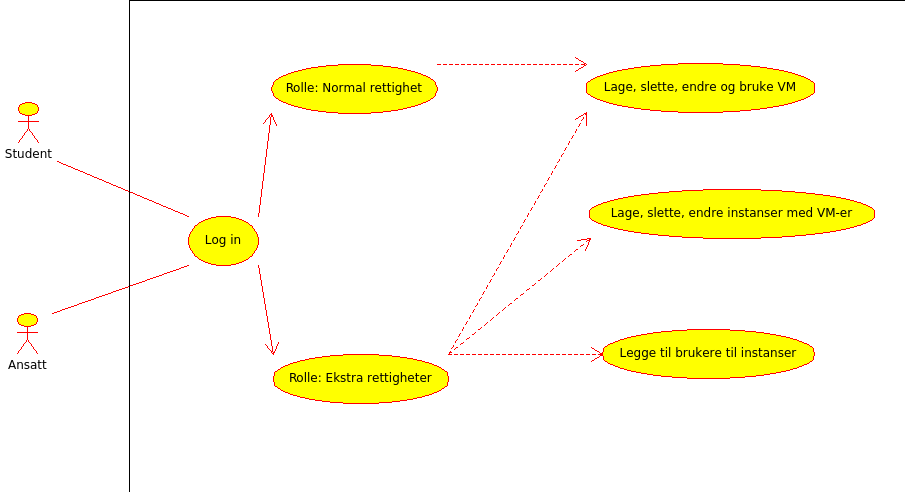
\includegraphics[width=100mm,height=90mm]{bilder/use_case_diagram}}
      \caption{\label{fig:usecase} Use case diagram 1}
\end{figure}

\begin{figure}[H]
	\center{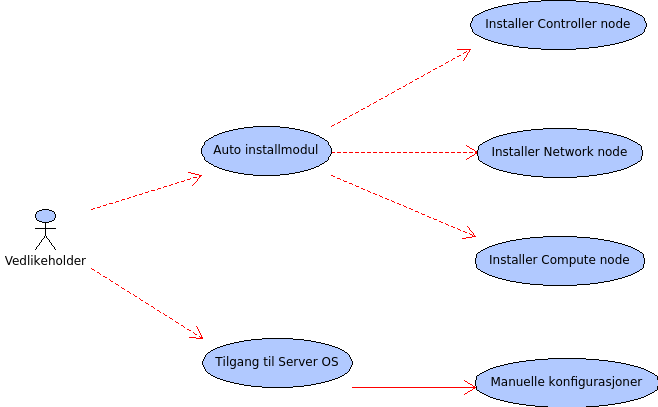
\includegraphics[width=100mm,height=90mm]{bilder/use_case_diagram_2}}
    \caption{\label{fig:usecase2} Use case diagram 2}
\end{figure}

\clearpage
\subsection{Høynivå use case}
\begin{table}[H]
	\begin{tabular}[Figur 1]{| p{1cm} | p{3cm} | p{3cm} | p{3cm} | p{2cm} }
		\hline \rowcolor{lightgray} \textbf{Use case ID} & \textbf{Usecase-navn} & \textbf{aktør} & \textbf{Kompleksitet} & \textbf{Prioritet} \\
		\hline \rowcolor{darkgray} 1 & Log in & Student og ansatt & Høy & 1 \\
		\hline \rowcolor{lightgray} 2 & Rolle: Normal rettighet & Student og ansatt & Middels & 2 \\
		\hline \rowcolor{darkgray} 3 & Rolle: Ekstra rettighet & Noen ansatte & Middels & 2 \\
		\hline \rowcolor{lightgray} 4 & Konfigurere VM-er & Lav & Studenter og ansatte & 2 \\
		\hline \rowcolor{darkgray} 5 & Konfigurere VM-instanser & Noen ansatte & Lav & 2 \\
		\hline \rowcolor{lightgray} 6 & Administrere VM-instanser & Noen ansatte & Middels & 3 \\
		\hline \rowcolor{darkgray} 7 & Auto install-modul & Vedlikeholder & Lav & 3 \\
		\hline \rowcolor{lightgray} 8 & Installer Controller node & Vedlikeholder & Lav & 3 \\
		\hline \rowcolor{darkgray} 9 & Installer Network node & Vedlikeholder & Lav & 3 \\
		\hline \rowcolor{lightgray} 10 & Installer Compute node & Vedlikeholder & Lav & 3 \\
		\hline \rowcolor{darkgray} 11 & Tilgang til server-OS & Vedlikeholder & Lav & 3 \\
		\hline \rowcolor{lightgray} 12 & Manuelle konfigurasjoner & Vedlikeholder & Lav & 3 \\
		\hline
	\end{tabular}
\end{table}

\begin{table}[H]
	\begin{tabular}[Figur 2]{| p{2cm} | p{9cm} |}
		\hline \rowcolor{lightgray} \textbf{Use case ID} & 1 \\
		\hline \rowcolor{darkgray} \textbf{Use case navn} & Log in \\
		\hline \rowcolor{lightgray} \textbf{aktør} & Ansatt og student\\
		\hline \rowcolor{darkgray} \textbf{Beskrivelse} & En bruker prøver å logge seg inn på SkyHiGh. Denne tar imot brukernavn og passord, samt innformasjon om fylke. \\
		\hline
	\end{tabular}
\end{table}

\begin{table}[H]
	\begin{tabular}[Figur 3]{| p{2cm} | p{9cm} |}
		\hline \rowcolor{lightgray} \textbf{Use case ID} & 2 \\
		\hline \rowcolor{darkgray} \textbf{Use case navn} & Rolle: Normal rettighet \\
		\hline \rowcolor{darkgray} \textbf{aktør} & Ansatt og student\\
		\hline \rowcolor{lightgray} \textbf{Beskrivelse} & Med innloggingsinformasjonen til brukeren vil autentiseringsprosessen avgjøre hvilke rettigheter brukeren har. \\
		\hline
	\end{tabular}
\end{table}

\begin{table}[H]
	\begin{tabular}[Figur 4]{| p{2cm} | p{9cm} |}
		\hline \rowcolor{lightgray} \textbf{Use case ID} & 3 \\
		\hline \rowcolor{darkgray} \textbf{Use case navn} & Rolle: Ekstra rettigheter \\
		\hline \rowcolor{lightgray} \textbf{aktør} & Noen ansatte\\
		\hline \rowcolor{darkgray} \textbf{Beskrivelse} & Med innloggingsinformasjonen til brukeren vil autentiseringsprosessen avgjøre hvilke rettigheter brukeren har. \\
		\hline
	\end{tabular}
\end{table}

\begin{table}[H]
	\begin{tabular}[Figur 5]{| p{2cm} | p{9cm} |}
		\hline \rowcolor{lightgray} \textbf{Use case ID} & 4 \\
		\hline \rowcolor{darkgray} \textbf{Use case navn} & Konfigurere VM-er \\
		\hline \rowcolor{lightgray} \textbf{aktør} & Ansatt og student\\
		\hline \rowcolor{darkgray} \textbf{Beskrivelse} & Her kan de brukeren lage, endre, slette og bruke VM-er. Her er det restriksjoner på ytelse og menge plass utifra hvilken rettighet brukeren har. \\
		\hline
	\end{tabular}
\end{table}

\begin{table}[H]
	\begin{tabular}[Figur 6]{| p{2cm} | p{9cm} |}
		\hline \rowcolor{lightgray} \textbf{Use case ID} & 5 \\
		\hline \rowcolor{darkgray} \textbf{Use case navn} & Konfigurere instanser med VM-er \\
		\hline \rowcolor{lightgray} \textbf{aktør} & Noen ansatte\\
		\hline \rowcolor{darkgray} \textbf{Beskrivelse} & Brukeren kan lage, endre, slette og bruke instanser med VM-er. \\
		\hline
	\end{tabular}
\end{table}

\begin{table}[H]
	\begin{tabular}[Figur 7]{| p{2cm} | p{9cm} |}
		\hline \rowcolor{lightgray} \textbf{Use case ID} & 6 \\
		\hline \rowcolor{darkgray} \textbf{Use case navn} & Administrere VM-instanser \\
		\hline \rowcolor{lightgray} \textbf{aktør} & Noen ansatte\\
		\hline \rowcolor{darkgray} \textbf{Beskrivelse} & Her har brukeren lov til å administrere de forskjellige instansene med VM-er. \\
		\hline
	\end{tabular}
\end{table}

\begin{table}[H]
	\begin{tabular}[Figur 2]{| p{2cm} | p{9cm} |}
		\hline \rowcolor{lightgray} \textbf{Use case ID} & 7 \\
		\hline \rowcolor{darkgray} \textbf{Use case navn} & Auto installmodul \\
		\hline \rowcolor{lightgray} \textbf{aktør} & Vedlikeholder\\
		\hline \rowcolor{darkgray} \textbf{Beskrivelse} & Denne modulen består enten at installerings-scriptet blir hentet fra en server, eller så er det en usbpinne som har tre forskjellige installeringer. Da er det bare å velge rett installering til rett modul i Openstack man skal installere. \\
		\hline
	\end{tabular}
\end{table}

\begin{table}[H]
	\begin{tabular}[Figur 2]{| p{2cm} | p{9cm} |}
		\hline \rowcolor{lightgray} \textbf{Use case ID} & 8 \\
		\hline \rowcolor{darkgray} \textbf{Use case navn} & Installer Controller node \\
		\hline \rowcolor{lightgray} \textbf{aktør} & Vedlikeholder \\
		\hline \rowcolor{darkgray} \textbf{Beskrivelse} & Script som kjører installasjonen av Controller noden. \\ 
		\hline
	\end{tabular}
\end{table}

\begin{table}[H]
	\begin{tabular}[Figur 2]{| p{2cm} | p{9cm} |}
		\hline \rowcolor{lightgray} \textbf{Use case ID} & 9 \\
		\hline \rowcolor{darkgray} \textbf{Use case navn} & Installer Network node\\
		\hline \rowcolor{lightgray} \textbf{aktør} & Vedlikeholder \\
		\hline \rowcolor{darkgray} \textbf{Beskrivelse} & Script som kjører installasjonen av Network noden. \\
		\hline	
	\end{tabular}
\end{table}

\begin{table}[H]
	\begin{tabular}[Figur 2]{| p{2cm} | p{9cm} |}
		\hline \rowcolor{lightgray} \textbf{Use case ID} & 10 \\
		\hline \rowcolor{darkgray} \textbf{Use case navn} & Installer Compute node \\
		\hline \rowcolor{lightgray} \textbf{aktør} & Vedlikeholder \\
		\hline \rowcolor{darkgray} \textbf{Beskrivelse} & Script som kjører installasjonen av Commpute noden. \\
		\hline	
	\end{tabular}
\end{table}

\begin{table}[H]
	\begin{tabular}[Figur 2]{| p{2cm} | p{9cm} |}
		\hline \rowcolor{lightgray} \textbf{Use case ID} & 11 \\
		\hline \rowcolor{darkgray} \textbf{Use case navn} & Tilgang til server-OS-et \\
		\hline \rowcolor{lightgray} \textbf{aktør} & Vedlikeholder \\
		\hline \rowcolor{darkgray} \textbf{Beskrivelse} & Dette er direkte tilgang til serverne. \\
		\hline
	\end{tabular}
\end{table}

\begin{table}[H]
	\begin{tabular}[Figur 2]{| p{2cm} | p{9cm} |}
		\hline \rowcolor{lightgray} \textbf{Use case ID} & 12 \\
		\hline \rowcolor{darkgray} \textbf{Use case navn} & Manuell konfigurasjon \\
		\hline \rowcolor{lightgray} \textbf{aktør} & Vedlikeholder \\
		\hline \rowcolor{darkgray} \textbf{Beskrivelse} & Dette er hvis vedlikeholder trenger å installere noe mer på serveren eller konfigurere noe. \\
		\hline
	\end{tabular}
\end{table}
\subsection{Detaljert use case}
\begin{figure}[H]
	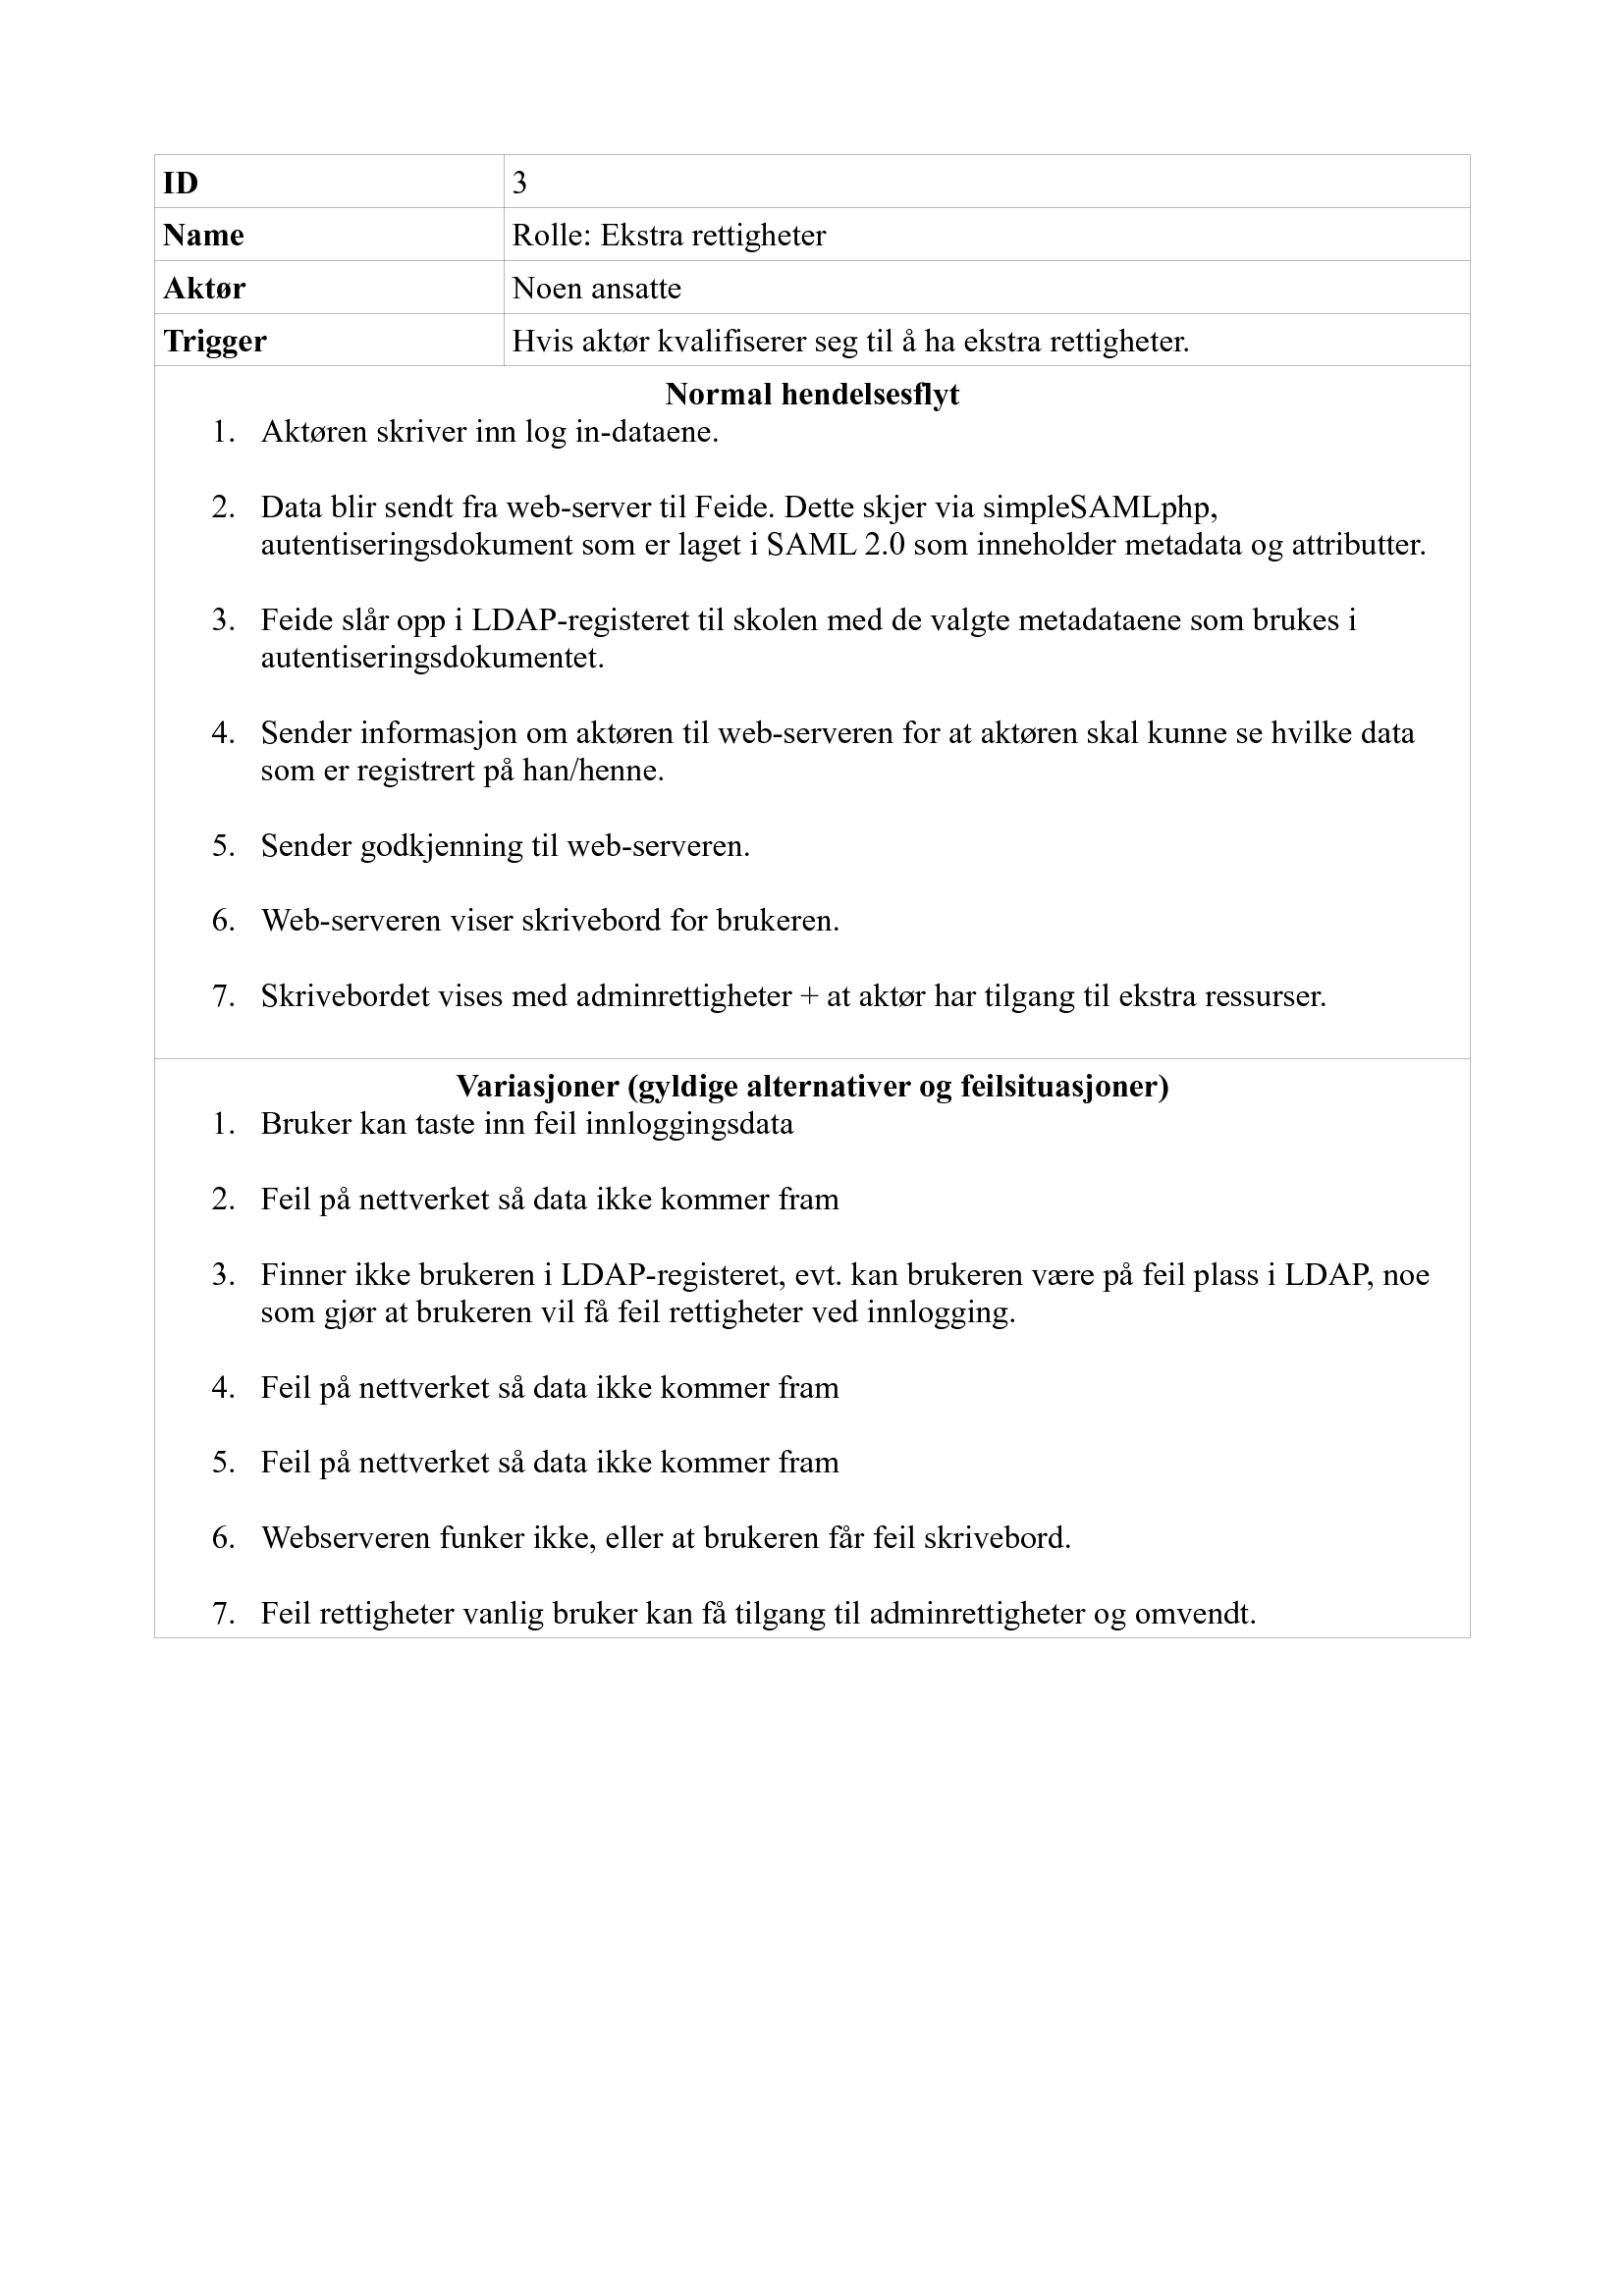
\includegraphics[height=280mm,width=150mm]{bilder/detaljert_usecase1}
	\caption{\label{fig:det_usecase1} Detaljert usecase}
\end{figure}
\newpage
\begin{figure}[H]
	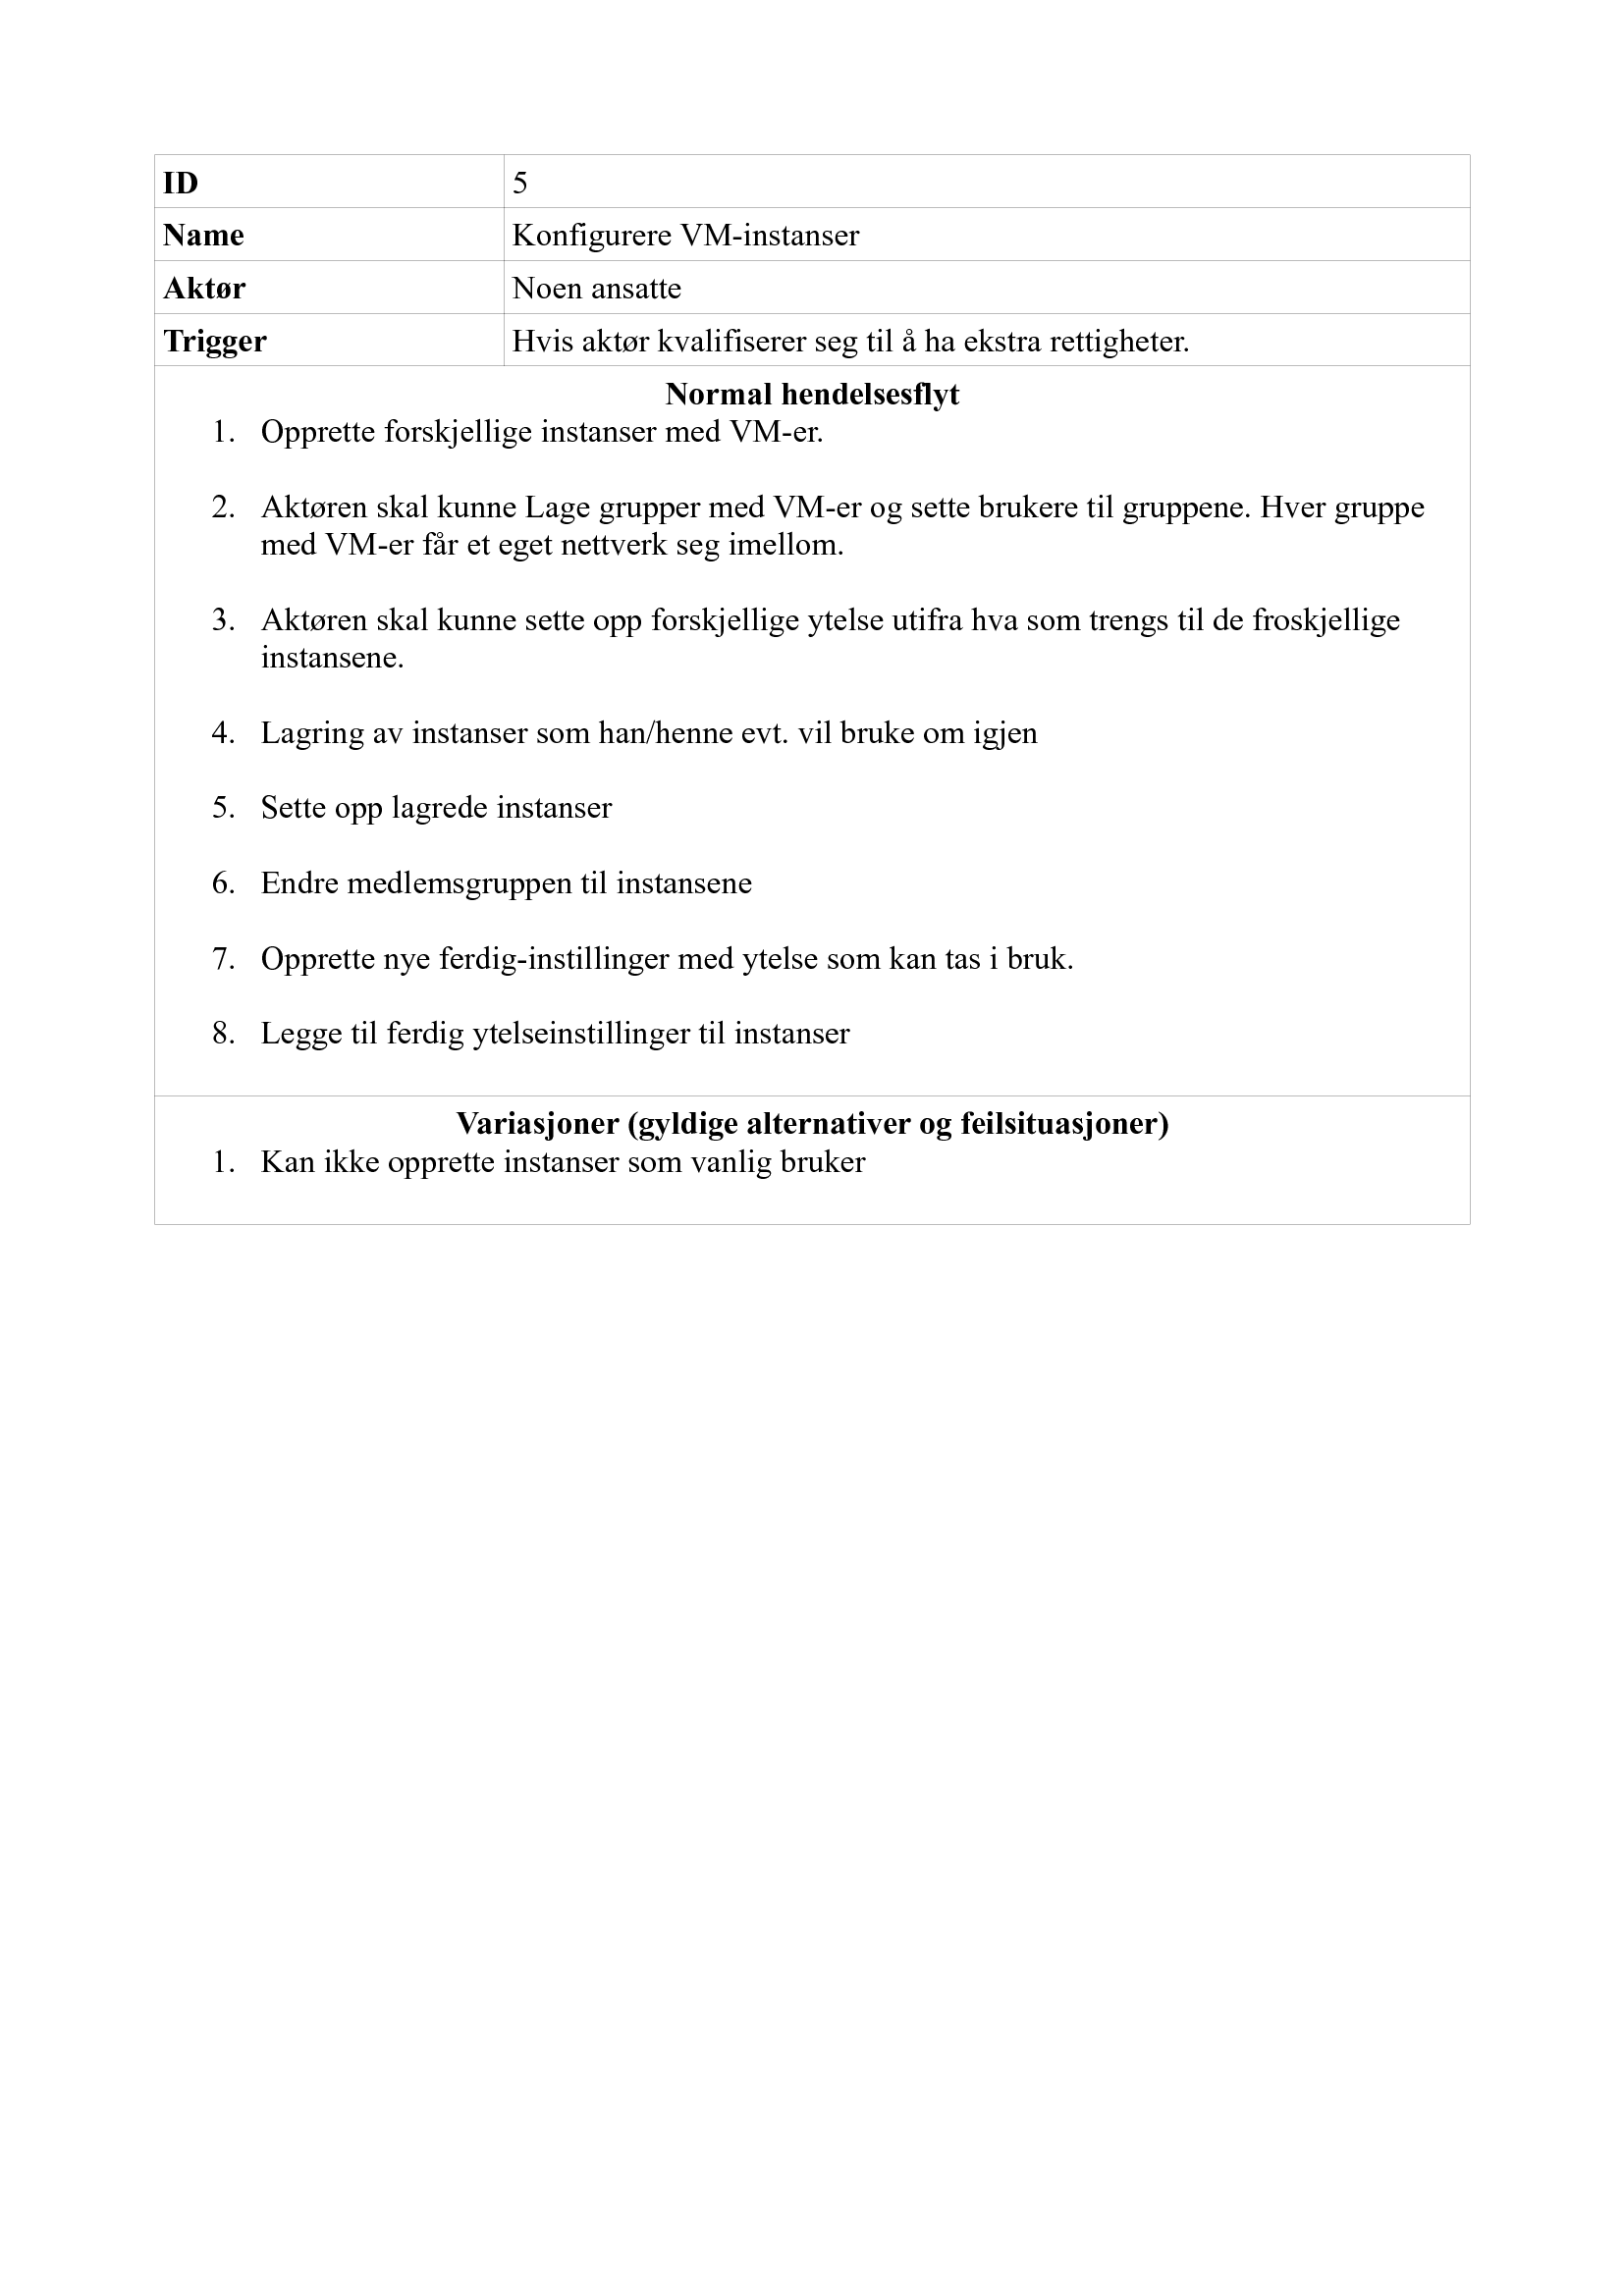
\includegraphics[height=280mm,width=150mm]{bilder/detaljert_usecase2}
	\caption{\label{fig:det_usecase2} Detaljert usecase}
\end{figure}
\newpage
\begin{figure}[H]
	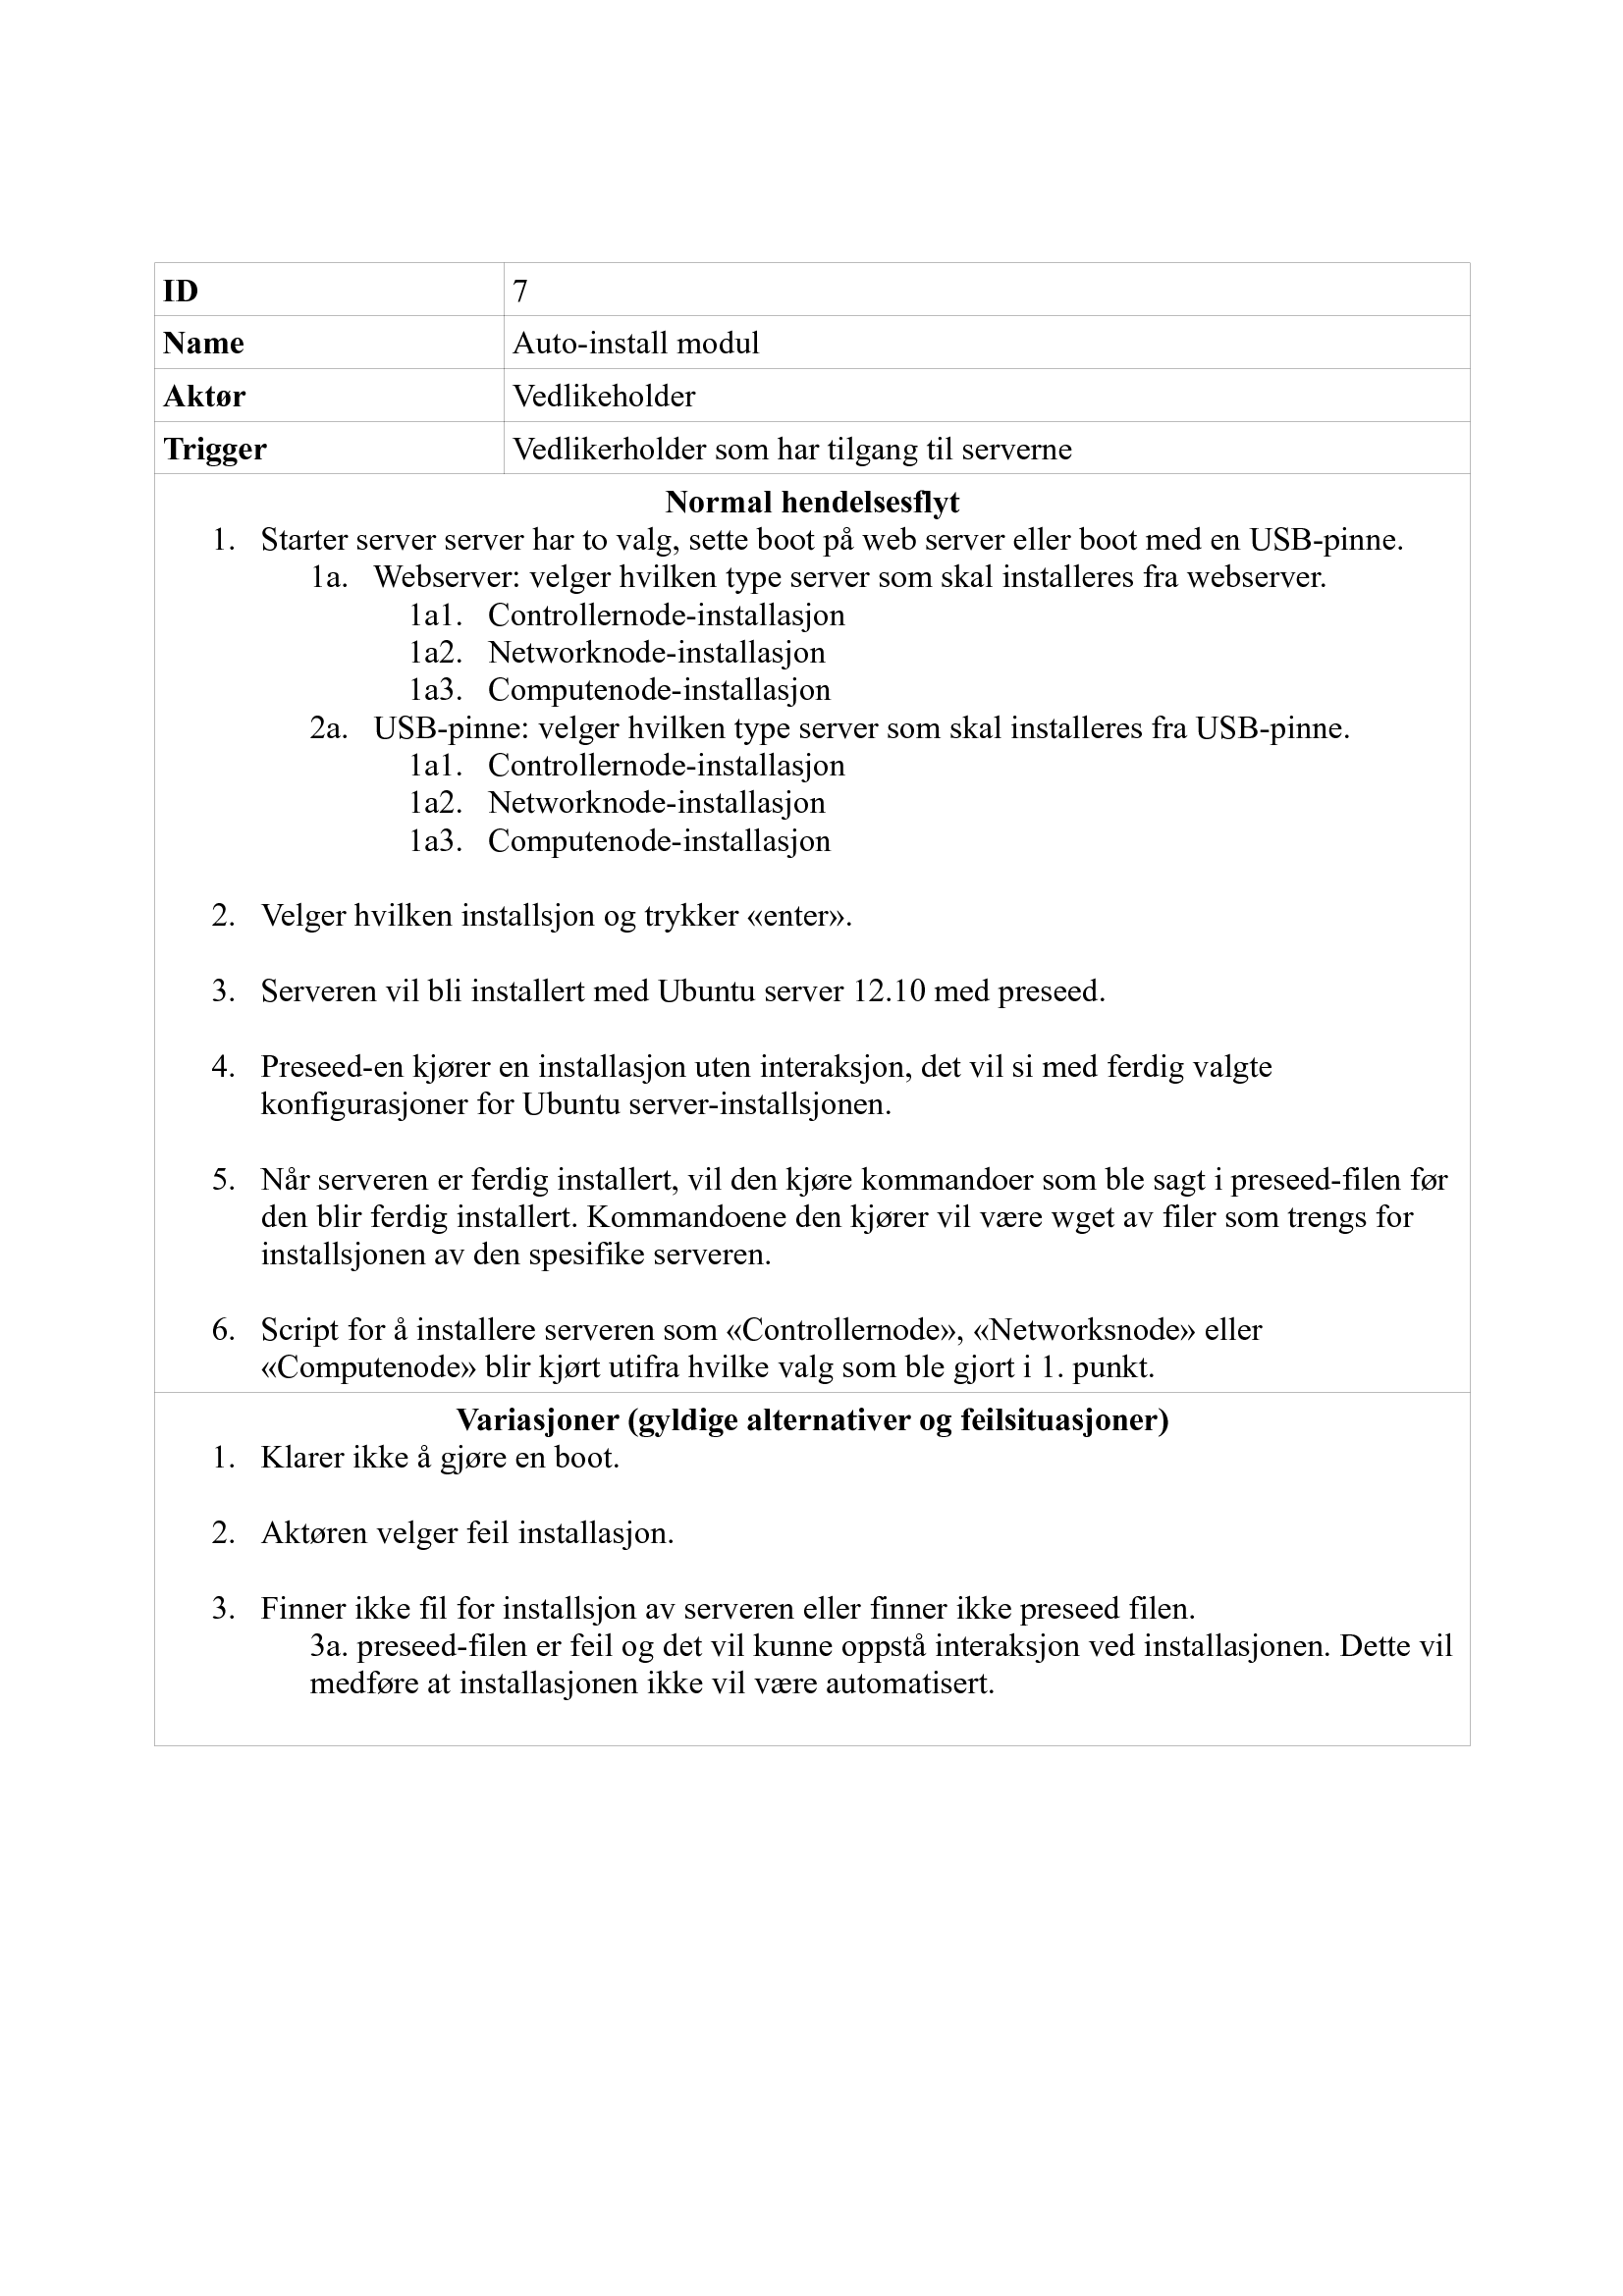
\includegraphics[height=280mm,width=150mm]{bilder/detaljert_usecase3}
    \caption{\label{fig:det_usecase3} Detaljert usecase}
\end{figure}

\clearpage
\subsection{Funksjon}
\begin{figure}[H]
      \center{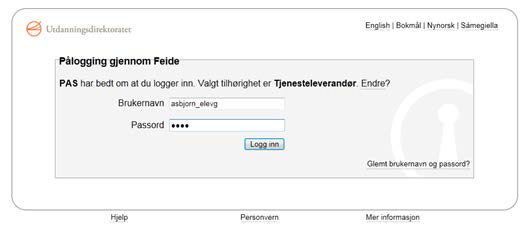
\includegraphics[height=50mm,width=100mm]{bilder/Palogging_via_Feide}}
      \caption{\label{fig:Pålogging_via_feide} Et eksempel på innlogging med feide}
\end{figure}
På figuren over kan du se hva som møter brukeren. På dette stadiet er det kun to datatyper, det er brukernavn og passord. Hendelserscenarioet er som figuren under.
\begin{figure}[H]
	\center{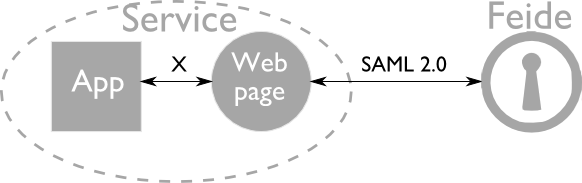
\includegraphics[scale=0.5]{bilder/innlogging-skjematisk}}
	\caption{\label{fig:Innlogging_skjematisk} Hvordan autentiseringen foregår}
\end{figure}
Webserveren er på kontrollernoden, Openstack-systemet er det vi kan referere til som appen på figuren over. Horizon er den som refereres til som “web page” på figuren, det er her vi skal lage innloggingsskjermen som vist på første figur.
\begin{description}
	\item{\tab •} Input - Brukernavn og passord fra brukeren. \\Skriver inn info, info-en blir sendt videre til Feide som er autentiseringsdatabase. Feide skjekker om bruker har tilgang og hvilken rolle brukeren har. Sender deretter info tilbake til “web page-en”.
	\item{\tab •} Output - Enten får brukeren at passord og brukernavn er feil, eller så kommer brukeren seg inn. Da vil brukergrensesnittet på Horizon vise seg for brukeren og brukeren kan lage, endre, slette og bruke VM-er utifra hvilken rolle/autentisering brukeren har.
\end{description}

\newpage
\subsection{Struktur og tverr-relasjoner}
\begin{figure}[H]
	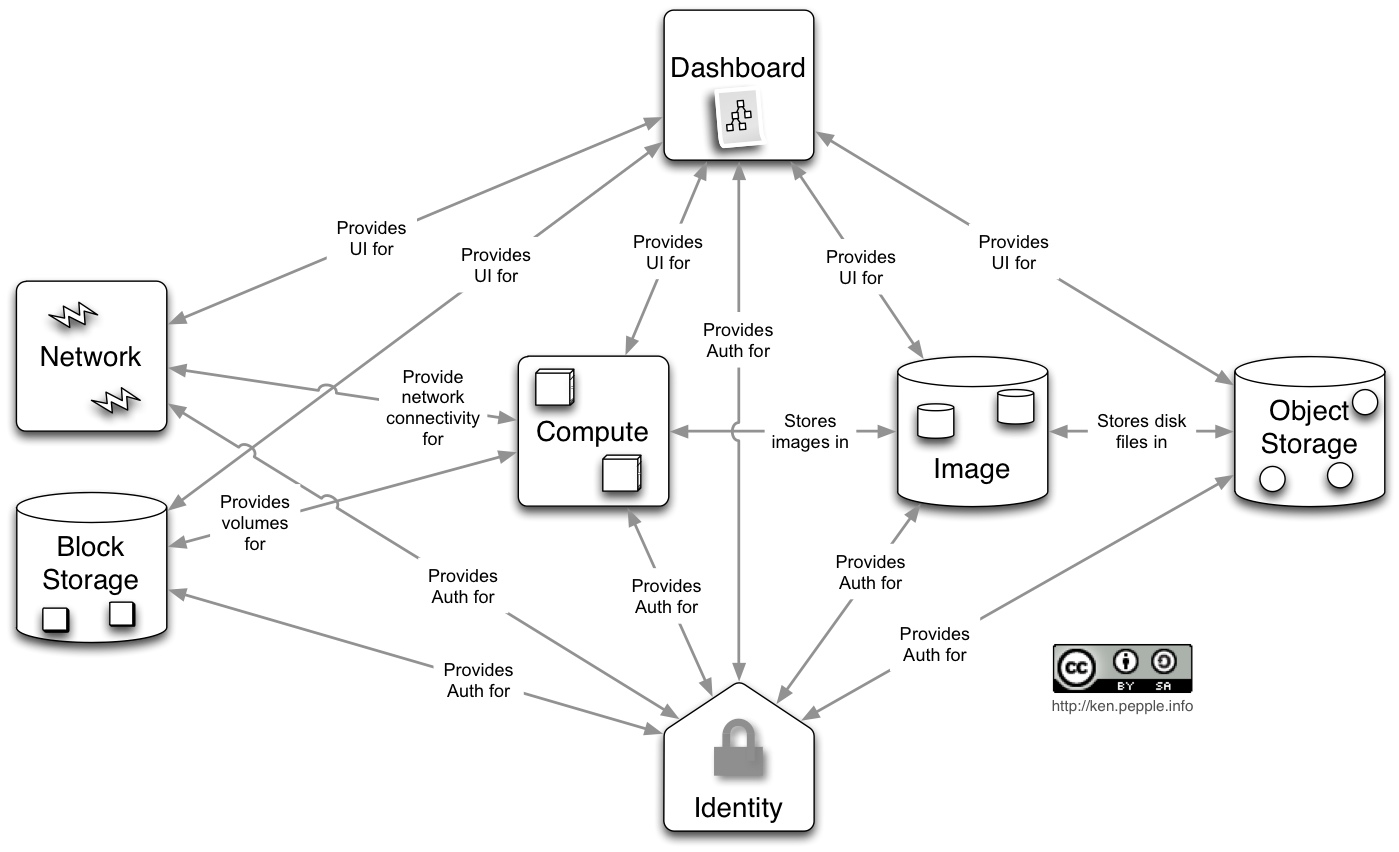
\includegraphics[width=150mm,height=100mm]{bilder/arkitektur_folsom}
	\caption{\label{fig:Struktur og tverr-relasjoner} Hvor går autentiseringstrafikken}
\end{figure}
Som du kan se på figuren over så går all autentifikasjon mellom dashboard og identity. Dashboard er Horizon og identity er Keystone. Horizon har kun autentisering mot keystone, det vil si at all vesentlig autentiseringsdata som keystone får går til Horizon. \newline \newline
Vi skjønner ut fra figuren, for at å autentisere mot FEIDE, så må vi vite hvilke data som kommer fra keystone. Når vi vet om de, så vet vi også hvilke data vi skal sende videre fra Horizon til FEIDE, utenom de obligatoriske attributtene (). 